\section{Logical Operations on Graph States}
\label{Sec:log_operation_graph}

In \cref{chap:2_qubit_gates}, we delved into the protocols employed to implement two-qubit gates on our device.
Additionally, we explored the constraints that limit our ability to execute certain other gate operations.

This section provides a deeper exploration of gates applied to graph states. 
Frequently, rather than directly applying the specific gate, we utilize an alternative operation that produces an equivalent effect for a particular initial state.

For instance, the Hadamard gate $H$ and a $\pi / 2$ rotation around the $y$ axis are different gates, as we can see from the different unitary matrices
\begin{equation}
    H = \frac{1}{\sqrt{2}}
    \begin{bmatrix}
        1 & 1 \\
        1 & -1
    \end{bmatrix} , \quad
    R_y(\pi / 2) = \frac{1}{\sqrt{2}}
    \begin{bmatrix}
        1 & -1 \\
        1 & 1
    \end{bmatrix} .
\end{equation}

However, when these gates are applied to the initial state $\ket{0}$, they yield identical resulting states:
\begin{equation}
    H \ket{0} = R_y(\pi/2) \ket{0} = \ket{+} .
\end{equation}

In our experiments, we frequently opt to replace Hadamard gates with rotations around the $x$, $y$, and $z$ axes. 
This choice is motivated by the considerable difficulty involved in implementing Hadamard gates.
Additionally, given our knowledge of the input state, we often find it feasible to substitute Hadamard gates with simpler gates that yield the same output state.

However, we need to be cautious as substituting all Hadamard gates with $\pi / 2$ rotations around the $y$ axis might not cover all situations. 
Take, for instance, the following:
\begin{equation}
    H H \ket{0} \neq
    R_y(\pi / 2) R_y(\pi / 2) \ket{0} .
\end{equation}

To ensure this equality holds, we need to alternate rotations of $\pi /2$ and $-\pi / 2$, as follows:
\begin{equation}
    H H \ket{0} =
    R_y(- \pi / 2) R_y(\pi / 2) \ket{0} .
\end{equation}

Now, let us revisit the two-qubit gates covered in \cref{chap:2_qubit_gates}: CZ, SWAP, and CNOT.
We will analyze their implementation methods to achieve the intended graph state as the final outcome.

\subsection{CZ}

The simplest among these gates is the CZ gate, given that graph states are formulated based on this specific gate. 
If our goal is to obtain the state depicted in \cref{fig:CZ_graph} as an outcome, we aim to execute operations on the qubits such as:
\begin{equation}
    \begin{quantikz}
      \lstick{$\ket{0}_1$} & \gate{H} & \ctrl{1} & \qw \\
      \lstick{$\ket{0}_2$} & \gate{H} & \control{} & \qw
    \end{quantikz}
\end{equation}
Fortunately, replacing the Hadamard gates with $\pi/2$ rotations around the $y$ axis for both qubits accomplishes this task:
\begin{equation}
    \begin{quantikz}
      \lstick{$\ket{0}_1$} & \gate{Y_+} & \ctrl{1} & \qw \\
      \lstick{$\ket{0}_2$} & \gate{Y_+} & \control{} & \qw
    \end{quantikz}
\end{equation}

\begin{figure}
    \centering
    

\tikzset{every picture/.style={line width=0.75pt}} %set default line width to 0.75pt        

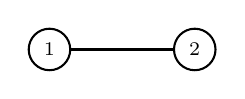
\begin{tikzpicture}[x=0.75pt,y=0.75pt,yscale=-1,xscale=1]
%uncomment if require: \path (0,162); %set diagram left start at 0, and has height of 162

%Shape: Circle [id:dp33085044400227215] 
\draw   (50,60) .. controls (50,54.48) and (54.48,50) .. (60,50) .. controls (65.52,50) and (70,54.48) .. (70,60) .. controls (70,65.52) and (65.52,70) .. (60,70) .. controls (54.48,70) and (50,65.52) .. (50,60) -- cycle ;
%Shape: Circle [id:dp45632065494671825] 
\draw   (120,60) .. controls (120,54.48) and (124.48,50) .. (130,50) .. controls (135.52,50) and (140,54.48) .. (140,60) .. controls (140,65.52) and (135.52,70) .. (130,70) .. controls (124.48,70) and (120,65.52) .. (120,60) -- cycle ;
%Straight Lines [id:da6274751888831748] 
\draw    (70,60) -- (120,60) ;

% Text Node
\draw (60,60) node  [font=\scriptsize]  {$1$};
% Text Node
\draw (130,60) node  [font=\scriptsize]  {$2$};


\end{tikzpicture}
    \vspace{-1cm}
    \caption{2-qubits linear graph}
    \label{fig:CZ_graph}
\end{figure}

From now on, we will use the following notation:
\begin{equation*}
    \begin{quantikz}
        \qw & \gate{Y_+} & \qw
    \end{quantikz}
    : R_y(+\pi/2) \, , \quad
    \begin{quantikz}
        \qw & \gate{Y_-} & \qw
    \end{quantikz}
    : R_y(-\pi/2) .
\end{equation*}

\subsection{SWAP}

When studying the SWAP gate, it's crucial to consider its impact on the entanglement between the qubits involved and their connections to other qubits.
If our aim is to replicate the functionality of the following circuit
\begin{equation}
\label{eq:SWAP_circuit}
    \begin{quantikz}
      \lstick{$\ket{0}_1$} & \gate{H} & \ctrl{1}   & \qw      & \qw \\
      \lstick{$\ket{0}_2$} & \gate{H} & \control{} & \swap{1} & \qw \\
      \lstick{$\ket{0}_3$} & \gate[style={fill=blue!10}]{H} & \qw        & \targX{} & \qw
    \end{quantikz}
\end{equation}
we need to examine the changes occurring in the entanglement between qubits 1 and 2.
A visual representation is provided in \cref{fig:SWAP_graph}.
The SWAP gate effectively transfers the entanglement between the qubits, similarly to a simple swap in the numbering of the two qubits.

\begin{figure}
    \centering
    

\tikzset{every picture/.style={line width=0.75pt}} %set default line width to 0.75pt        

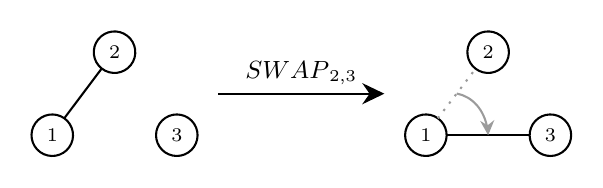
\begin{tikzpicture}[x=0.75pt,y=0.75pt,yscale=-1,xscale=1]
%uncomment if require: \path (0,162); %set diagram left start at 0, and has height of 162

%Shape: Circle [id:dp34495488497110016] 
\draw   (87.86,66.18) .. controls (84.45,70.52) and (78.17,71.28) .. (73.82,67.86) .. controls (69.48,64.45) and (68.72,58.17) .. (72.14,53.82) .. controls (75.55,49.48) and (81.83,48.72) .. (86.18,52.14) .. controls (90.52,55.55) and (91.28,61.83) .. (87.86,66.18) -- cycle ;
%Shape: Circle [id:dp2623874134924238] 
\draw   (41.84,94.21) .. controls (45.04,89.71) and (51.28,88.65) .. (55.79,91.84) .. controls (60.29,95.04) and (61.35,101.28) .. (58.16,105.79) .. controls (54.96,110.29) and (48.72,111.35) .. (44.21,108.16) .. controls (39.71,104.96) and (38.65,98.72) .. (41.84,94.21) -- cycle ;
%Shape: Circle [id:dp1378234889252382] 
\draw   (101.66,105.51) .. controls (98.61,100.91) and (99.88,94.7) .. (104.49,91.66) .. controls (109.09,88.61) and (115.3,89.88) .. (118.34,94.49) .. controls (121.39,99.09) and (120.12,105.3) .. (115.51,108.34) .. controls (110.91,111.39) and (104.7,110.12) .. (101.66,105.51) -- cycle ;
%Straight Lines [id:da18089547069059342] 
\draw    (73.82,67.86) -- (55.79,91.84) ;
%Shape: Circle [id:dp18245241155845826] 
\draw   (267.97,66.03) .. controls (264.64,70.44) and (258.37,71.31) .. (253.96,67.97) .. controls (249.56,64.64) and (248.69,58.37) .. (252.02,53.96) .. controls (255.36,49.56) and (261.63,48.69) .. (266.03,52.02) .. controls (270.44,55.36) and (271.31,61.63) .. (267.97,66.03) -- cycle ;
%Shape: Circle [id:dp8811036011863903] 
\draw   (221.84,94.21) .. controls (225.04,89.71) and (231.28,88.65) .. (235.78,91.84) .. controls (240.29,95.04) and (241.35,101.28) .. (238.15,105.78) .. controls (234.96,110.29) and (228.72,111.35) .. (224.21,108.15) .. controls (219.71,104.96) and (218.65,98.72) .. (221.84,94.21) -- cycle ;
%Straight Lines [id:da20903671041287875] 
\draw    (240,100) -- (280,100) ;
%Shape: Circle [id:dp9231143684580897] 
\draw   (281.82,105.75) .. controls (278.64,101.24) and (279.73,95) .. (284.24,91.82) .. controls (288.76,88.64) and (295,89.73) .. (298.18,94.24) .. controls (301.36,98.76) and (300.27,105) .. (295.75,108.18) .. controls (291.24,111.36) and (285,110.27) .. (281.82,105.75) -- cycle ;
%Straight Lines [id:da14252568592014891] 
\draw    (130,80) -- (207,80) ;
\draw [shift={(210,80)}, rotate = 180] [fill={rgb, 255:red, 0; green, 0; blue, 0 }  ][line width=0.08]  [draw opacity=0] (10.72,-5.15) -- (0,0) -- (10.72,5.15) -- (7.12,0) -- cycle    ;
%Straight Lines [id:da02595413260158763] 
\draw [color={rgb, 255:red, 155; green, 155; blue, 155 }  ,draw opacity=1 ] [dash pattern={on 0.84pt off 2.51pt}]  (235.78,91.84) -- (253.96,67.97) ;
%Curve Lines [id:da2796836261210731] 
\draw [color={rgb, 255:red, 155; green, 155; blue, 155 }  ,draw opacity=1 ]   (244.87,79.91) .. controls (252.27,81.36) and (258.18,87.56) .. (259.69,97.08) ;
\draw [shift={(260,100)}, rotate = 266.58] [fill={rgb, 255:red, 155; green, 155; blue, 155 }  ,fill opacity=1 ][line width=0.08]  [draw opacity=0] (7.14,-3.43) -- (0,0) -- (7.14,3.43) -- (4.74,0) -- cycle    ;

% Text Node
\draw (50,100) node  [font=\scriptsize]  {$1$};
% Text Node
\draw (80,60) node  [font=\scriptsize]  {$2$};
% Text Node
\draw (110,100) node  [font=\scriptsize]  {$3$};
% Text Node
\draw (230,100) node  [font=\scriptsize]  {$1$};
% Text Node
\draw (260,60) node  [font=\scriptsize]  {$2$};
% Text Node
\draw (290,100) node  [font=\scriptsize]  {$3$};
% Text Node
\draw (170,77) node [anchor=south] [inner sep=0.75pt]  [font=\small] [align=left] {$\displaystyle \text{SWAP}_{2,3}$};


\end{tikzpicture}
    \vspace{-1cm}
    \caption{Action of SWAP gate on entangling bonds with neighbouring qubits}
    \label{fig:SWAP_graph}
\end{figure}

Another aspect to consider is that we primarily implement the SWAP gate between a storage and an emitter. 
Consequently, in our example, we will define qubit 3 as the emitter qubit. 
This means we're unable to perform single-qubit gates on it due to its rapid state decay.
We can execute the SWAP gate of \cref{fig:SWAP_graph} and generate an analogue final state by running the following protocol
\begin{equation}
    \begin{quantikz}
      \lstick{$\ket{0}_1$} & \gate{Y_+} & \ctrl{1}   & \qw      & \qw                & \qw \\
      \lstick{$\ket{0}_2$} & \gate{Y_+} & \control{} & \swap{1} & \gate[style={fill=blue!10}]{Y_+} & \qw \\
      \lstick{$\ket{0}_3$} & \qw                & \qw        & \targX{} & \qw                & \qw
    \end{quantikz}
\end{equation}
In the circuit architecture, the SWAP gate basically transfers both the state and the entangling bonds from qubit 2 to qubit 3.
Consequently, to achieve the state represented in \cref{eq:SWAP_circuit}, we need to further apply a Hadamard gate (or a $y$ rotation) on qubit 2 to bring it to the state $\ket{+}$.

\subsection{CNOT}

The situation changes once more when dealing with the CNOT gate.
The following equivalence between the resulting quantum states can be easily checked:
\begin{equation}
    \begin{quantikz}
      \lstick{$\ket{0}_1$} & \gate{H} & \ctrl{2}   & \qw         & \qw \\
      \lstick{$\ket{0}_2$} & \gate{H} & \qw        & \ctrl{1}    & \qw \\
      \lstick{$\ket{0}_3$} & \gate{H} & \control{} & \control{}  & \qw
    \end{quantikz}
    \; = \;
    \begin{quantikz} 
      \lstick{$\ket{0}_1$} & \gate{H} & \ctrl{1}   & \qw      & \qw      & \qw \\
      \lstick{$\ket{0}_2$} & \gate{H} & \control{} & \ctrl{1} & \gate{H} & \qw \\
      \lstick{$\ket{0}_3$} & \qw      & \qw        & \targ{}  & \qw      & \qw
    \end{quantikz}
\end{equation}
Thus, the CNOT gate, followed by an Hadamard, effectively transfers all entanglement from the control qubit to the target qubit, while also entangling the two qubits, as depicted in \cref{fig:CNOT_graph}.

\begin{figure}
    \centering
    

\tikzset{every picture/.style={line width=0.75pt}} %set default line width to 0.75pt        

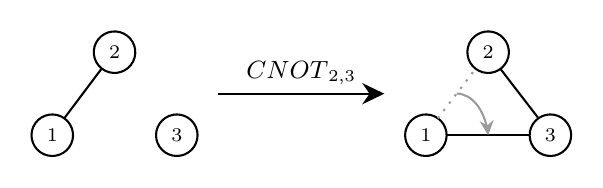
\begin{tikzpicture}[x=0.75pt,y=0.75pt,yscale=-1,xscale=1]
%uncomment if require: \path (0,162); %set diagram left start at 0, and has height of 162

%Shape: Circle [id:dp23417453743827976] 
\draw   (87.86,66.18) .. controls (84.45,70.52) and (78.17,71.28) .. (73.82,67.86) .. controls (69.48,64.45) and (68.72,58.17) .. (72.14,53.82) .. controls (75.55,49.48) and (81.83,48.72) .. (86.18,52.14) .. controls (90.52,55.55) and (91.28,61.83) .. (87.86,66.18) -- cycle ;
%Shape: Circle [id:dp011544140967992389] 
\draw   (41.84,94.21) .. controls (45.04,89.71) and (51.28,88.65) .. (55.79,91.84) .. controls (60.29,95.04) and (61.35,101.28) .. (58.16,105.79) .. controls (54.96,110.29) and (48.72,111.35) .. (44.21,108.16) .. controls (39.71,104.96) and (38.65,98.72) .. (41.84,94.21) -- cycle ;
%Shape: Circle [id:dp416194828283707] 
\draw   (101.66,105.51) .. controls (98.61,100.91) and (99.88,94.7) .. (104.49,91.66) .. controls (109.09,88.61) and (115.3,89.88) .. (118.34,94.49) .. controls (121.39,99.09) and (120.12,105.3) .. (115.51,108.34) .. controls (110.91,111.39) and (104.7,110.12) .. (101.66,105.51) -- cycle ;
%Straight Lines [id:da17802990060125945] 
\draw    (73.82,67.86) -- (55.79,91.84) ;
%Shape: Circle [id:dp026916354896634798] 
\draw   (267.97,66.03) .. controls (264.64,70.44) and (258.37,71.31) .. (253.96,67.97) .. controls (249.56,64.64) and (248.69,58.37) .. (252.02,53.96) .. controls (255.36,49.56) and (261.63,48.69) .. (266.03,52.02) .. controls (270.44,55.36) and (271.31,61.63) .. (267.97,66.03) -- cycle ;
%Shape: Circle [id:dp9684318791918579] 
\draw   (221.84,94.21) .. controls (225.04,89.71) and (231.28,88.65) .. (235.78,91.84) .. controls (240.29,95.04) and (241.35,101.28) .. (238.15,105.78) .. controls (234.96,110.29) and (228.72,111.35) .. (224.21,108.15) .. controls (219.71,104.96) and (218.65,98.72) .. (221.84,94.21) -- cycle ;
%Straight Lines [id:da43300710363321016] 
\draw    (265.93,68.05) -- (284.24,91.82) ;
%Shape: Circle [id:dp3103272610346469] 
\draw   (281.82,105.75) .. controls (278.64,101.24) and (279.73,95) .. (284.24,91.82) .. controls (288.76,88.64) and (295,89.73) .. (298.18,94.24) .. controls (301.36,98.76) and (300.27,105) .. (295.75,108.18) .. controls (291.24,111.36) and (285,110.27) .. (281.82,105.75) -- cycle ;
%Straight Lines [id:da6511414638961373] 
\draw    (130,80) -- (207,80) ;
\draw [shift={(210,80)}, rotate = 180] [fill={rgb, 255:red, 0; green, 0; blue, 0 }  ][line width=0.08]  [draw opacity=0] (10.72,-5.15) -- (0,0) -- (10.72,5.15) -- (7.12,0) -- cycle    ;
%Straight Lines [id:da1905731404703308] 
\draw    (240,100) -- (280,100) ;
%Straight Lines [id:da19331622592606712] 
\draw [color={rgb, 255:red, 155; green, 155; blue, 155 }  ,draw opacity=1 ] [dash pattern={on 0.84pt off 2.51pt}]  (235.78,91.84) -- (253.96,67.97) ;
%Curve Lines [id:da4343842529052825] 
\draw [color={rgb, 255:red, 155; green, 155; blue, 155 }  ,draw opacity=1 ]   (244.87,79.91) .. controls (252.59,80.17) and (257.91,88.06) .. (259.59,97.12) ;
\draw [shift={(260,100)}, rotate = 264.4] [fill={rgb, 255:red, 155; green, 155; blue, 155 }  ,fill opacity=1 ][line width=0.08]  [draw opacity=0] (7.14,-3.43) -- (0,0) -- (7.14,3.43) -- (4.74,0) -- cycle    ;

% Text Node
\draw (50,100) node  [font=\scriptsize]  {$1$};
% Text Node
\draw (80,60) node  [font=\scriptsize]  {$2$};
% Text Node
\draw (110,100) node  [font=\scriptsize]  {$3$};
% Text Node
\draw (230,100) node  [font=\scriptsize]  {$1$};
% Text Node
\draw (260,60) node  [font=\scriptsize]  {$2$};
% Text Node
\draw (290,100) node  [font=\scriptsize]  {$3$};
% Text Node
\draw (170,77) node [anchor=south] [inner sep=0.75pt]  [font=\small] [align=left] {$\displaystyle \text{CNOT}_{2,3}$};


\end{tikzpicture}
    \vspace{-1cm}
    \caption{Action of CNOT gate on the entangling bonds of the target qubit}
    \label{fig:CNOT_graph}
\end{figure}

It's worth noting that the equivalence is solely between outcomes, assuming the initial state is $\ket{000}$, not between the quantum circuits themselves.
In practice, the unitary matrices representing the actions of the two circuits would differ.

To replicate the action of this gate and achieve the same resulting graph state, precise attention must be paid to the phase signs in rotations around the $y$ axis.
We will maintain the assumption that qubit 3 serves as an emitter qubit, as previously established in the case of the SWAP gate.
The executable sequence of gates on our device is the following:
\begin{equation}
    \begin{quantikz}
      \lstick{$\ket{0}_1$} & \gate{Y_+}  & \ctrl{1}   & \qw         & \qw                 & \qw \\
      \lstick{$\ket{0}_2$} & \gate[style={fill=red!10}]{Y_-} & \control{} & \ctrl{1}    & \gate{Y_+} & \qw \\
      \lstick{$\ket{0}_3$} & \qw                 & \qw        & \targ{}     & \qw                 & \qw
    \end{quantikz}
\end{equation}

Typically, when multiple Hadamard gates are applied to the same qubit without resetting it through a SWAP gate with an emitter, it becomes necessary to alternate the rotation's sign around the $y$ axis.
Intuitively, this adjustment is needed because applying two rotations is not equivalent to applying two Hadamard gates, even when the initial state is $\ket{0}$.
To accurately represent this scenario, we might need to implement a sequence resembling the following:
\begin{equation}
    H H \ket{0} =
    R_y(- \pi / 2) R_y(\pi / 2) \ket{0} =
    R_y(\pi / 2) R_y(-\pi / 2) \ket{0} .
\end{equation}

Moreover, it's important to note that the effect of a $y$ rotation and the Hadamard gate differs when applied to the state $\ket{1}$:
\begin{equation}
    H \ket{1} = \ket{-} , \quad
    R_y(\pi / 2) \ket{1} = - \ket{-} .
\end{equation}

Hence, intuitively, it becomes crucial to alternate the signs of the $\pi/2$ rotation around the $y$ axis, ensuring that the final rotation within the sequence is positive. 
This alternating pattern ensures proper alignment with the intended quantum operations, particularly when dealing with sequences involving multiple rotations or Hadamard gates on the same qubit.